\newpage

\section*{ $^{90}$Zr(n,2n)$^{89}$Zr }

Power Level: 100 kW(th) \\
Time at Power: 60.0 m \\
Wait Time:  2.0 d \\
Counting Time: 60.0 m \\
Total Activity at Removal: 1.28e-05 $\mu Ci$

\begin{table*}[h]
\centering
\begin{tabular}{ |c|c|c|c|c|c| }
 \hline
 Position & Mass $mg$ & Counting Activity $\mu Ci$ & Area (Counts) & Error \% \\
 \hline 
 1 & 0.98 & 6.66e-06 & 2.24e+01 & 21.1160 \\ 
\hline
 2 & 0.98 & 3.42e-06 & 1.15e+01 & 29.4430 \\ 
\hline
 3 & 0.98 & 1.23e-07 & 4.13e-01 & 155.6290 \\ 
\hline
 4 & 0.98 & 2.38e-06 & 8.02e+00 & 35.3128 \\ 
\hline
\end{tabular}
\end{table*}

\begin{figure}[h]
\centering
\begin{subfigure}{.5\textwidth}
  \centering
     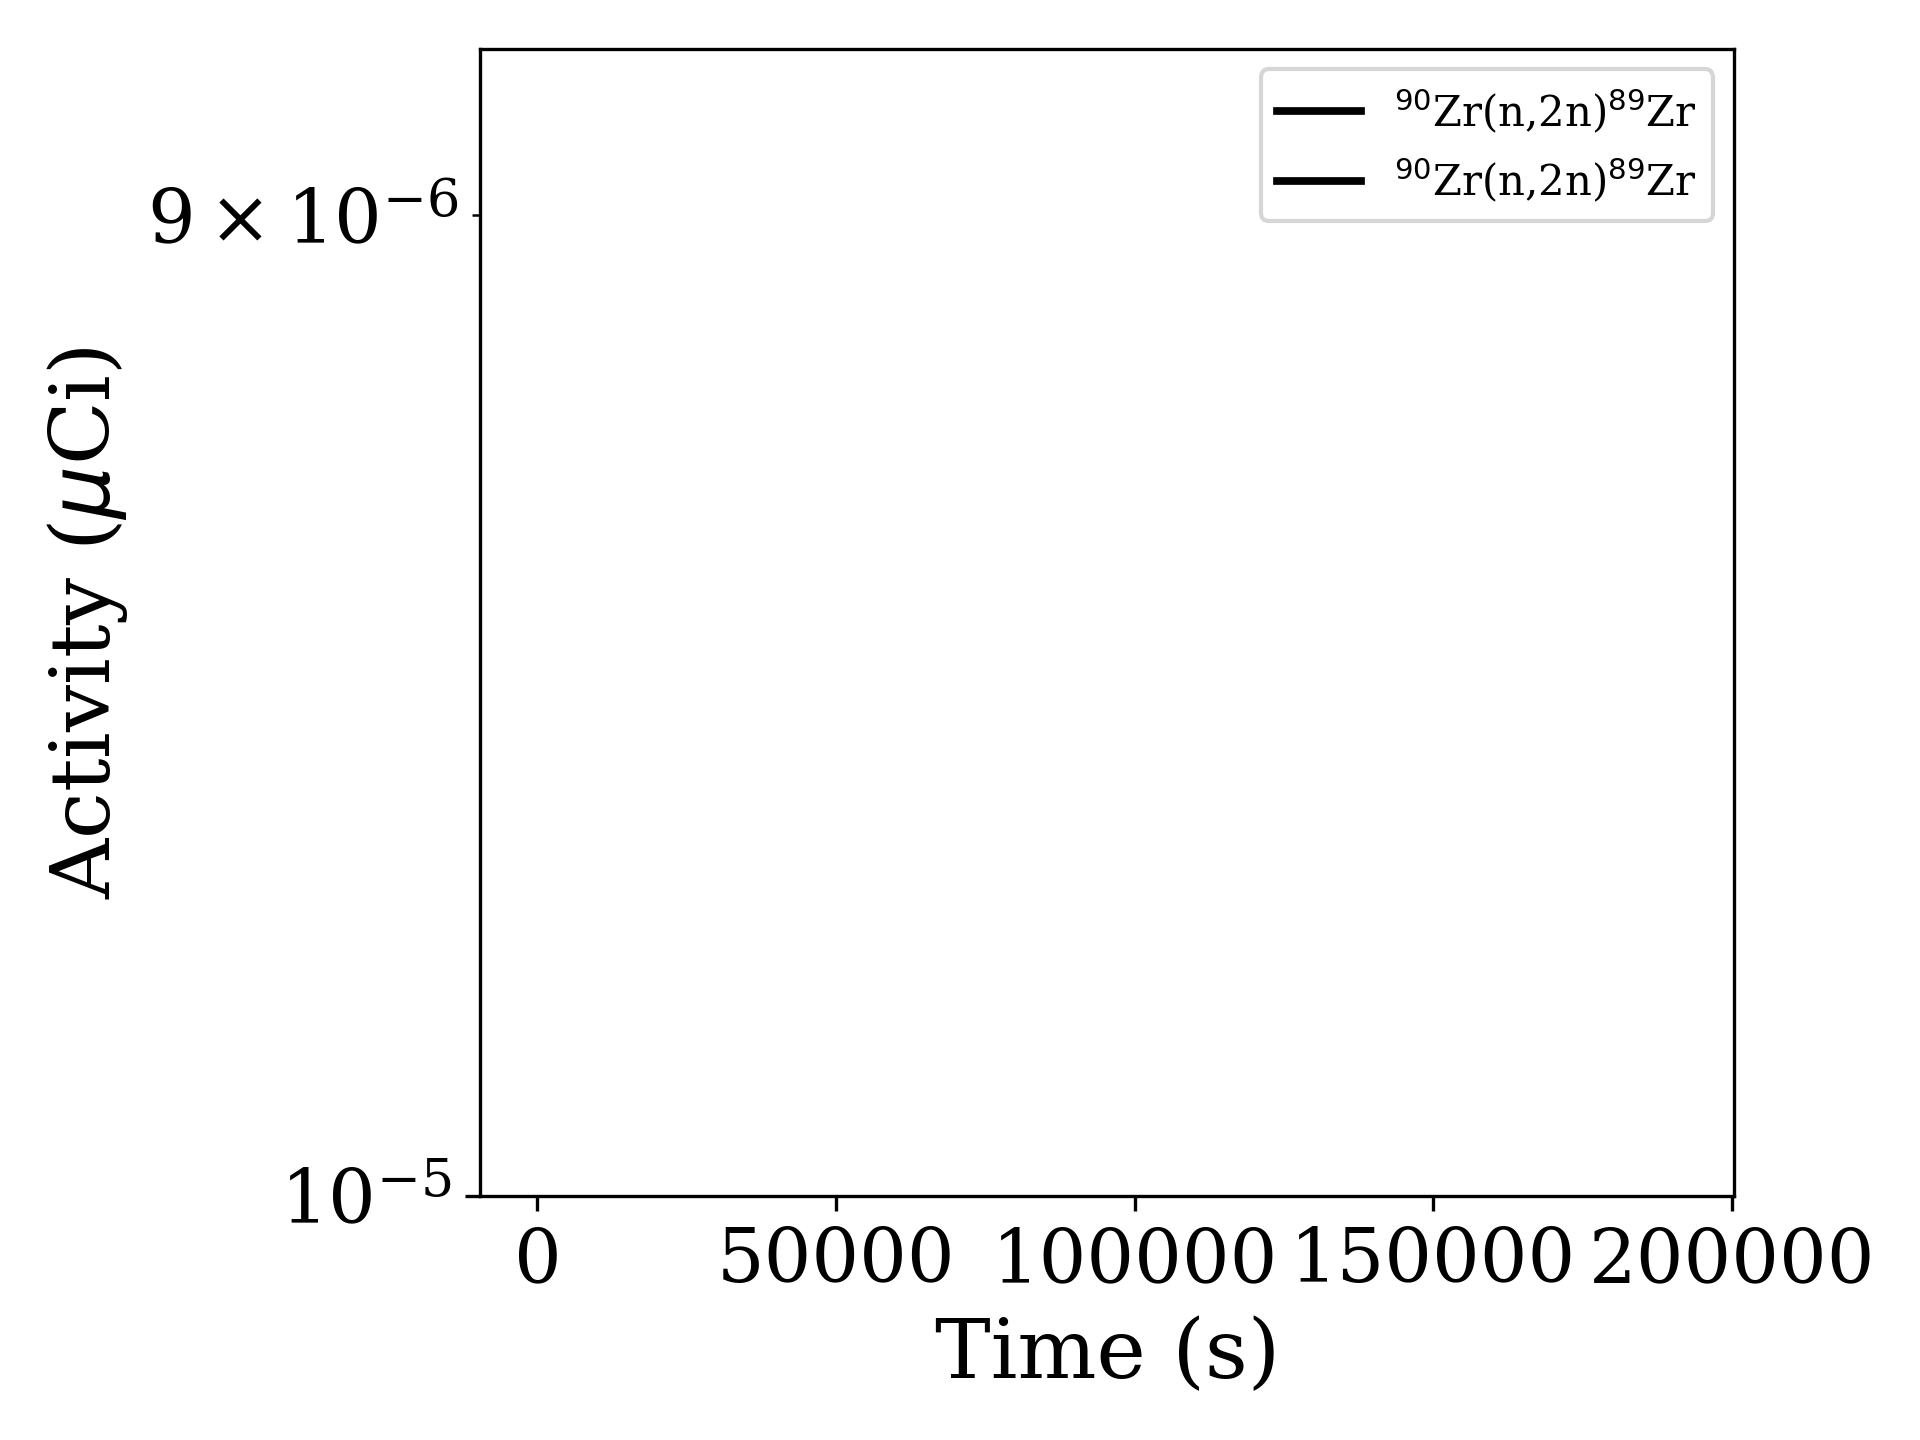
\includegraphics[width=.8\textwidth]{plot/Zr-90(n,2n)Zr-89_library1} 

  \caption{A subfigure}
  \label{fig:sub1}
\end{subfigure}%
\begin{subfigure}{.5\textwidth}
  \centering
     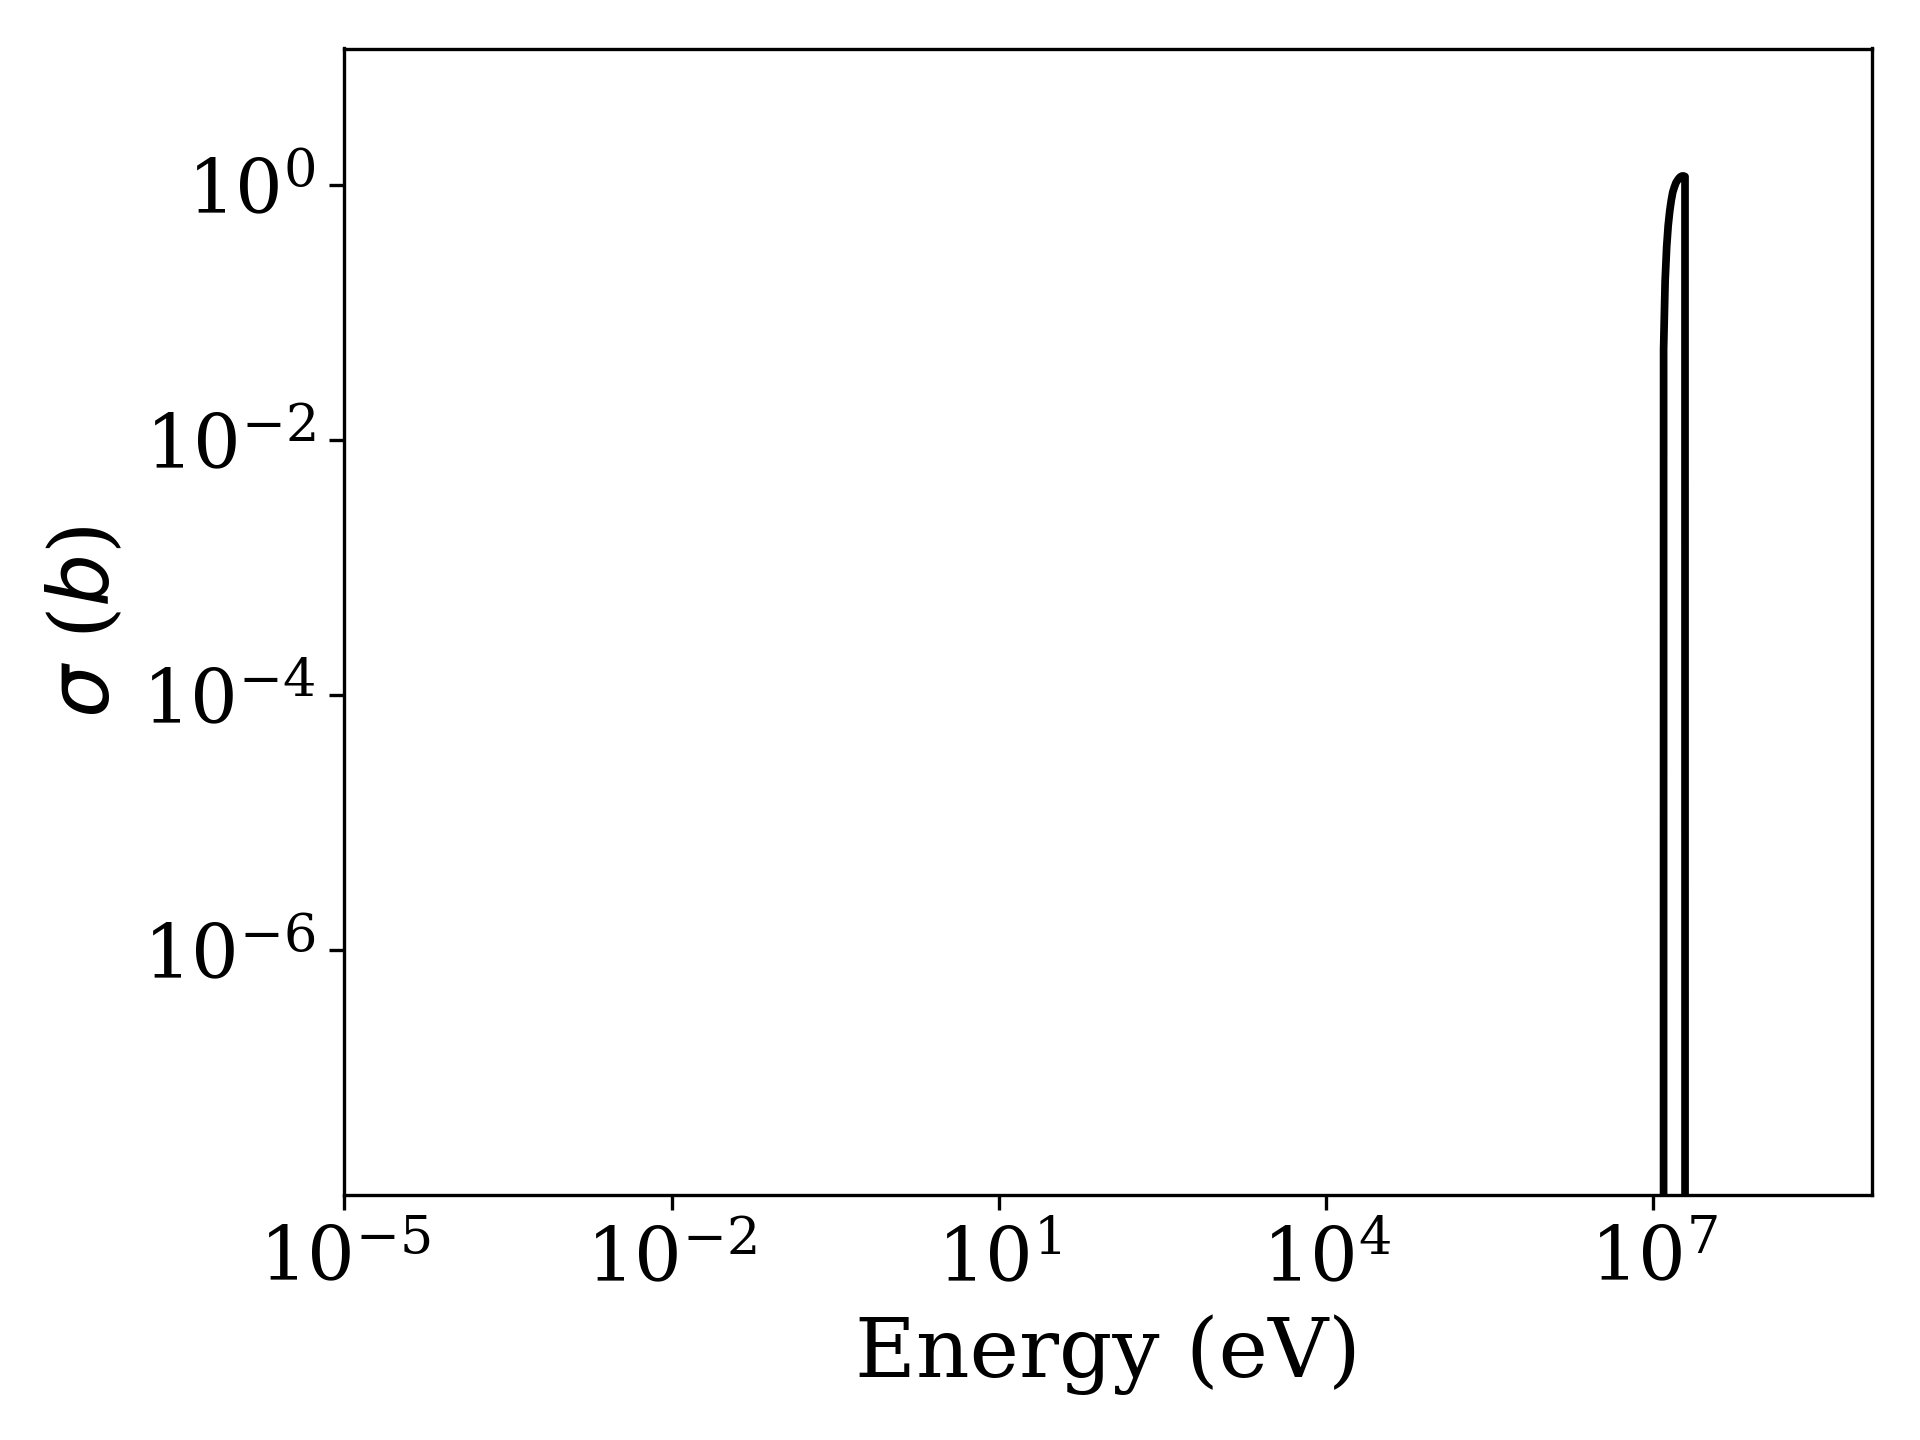
\includegraphics[width=.8\textwidth]{plot/Zr-90(n,2n)Zr-89} 

  \caption{A subfigure}
  \label{fig:sub2}
\end{subfigure}
\caption{A figure with two subfigures}
\label{fig:test}
\end{figure}

\begin{table*}[h]
\centering
\begin{tabular}{ |c|c|c|c|c|c|c| }
 \hline
 Reaction & T$_{1/2}$ & ROI (eV) & Important Gammas (keV) \\
 \hline 
 $^{90}$Zr(n,2n)$^{89}$Zr & 64.0 d & 1.25e+07, 1.39e+07 & 909.15(0.9904) \\ 
\hline
\end{tabular}
\end{table*}
